\documentclass[11pt]{scrartcl}
\usepackage[utf8]{inputenc}
\usepackage[sexy]{evanchen} 
\usepackage{graphicx}
\graphicspath{{8 Outsource K Math/Gambar/}}

\title{Inversi}
\author{Azzam and Akeyla}

\begin{document}

\maketitle

\section{Definisi}
Diberikan sebuah lingkaran $\omega$ yang berpusat di titik $O$ dan berjari-jari $R$. Notasikan pula $P_{\infty}$ sebagai titik di tak hingga. Inversi terhadap $\omega$ merupakan pemetaan semua titik $P$ di bidang berdasarkan aturan:
\begin{enumerate}
    \item Jika $P = O$, maka $P$ dipetakan ke $P_{\infty}$
    \item Jika $P = P_{\infty}$, maka $P$ dipetakan ke $O$
    \item Jika $P$ titik selain itu, maka $P$ dipetakan ke titik $P^{*}$ sedemikian hingga $O, P, P^{*}$ segaris dan $OP\cdot OP^{*} = R^2$
\end{enumerate}

\section{Properti}
Beberapa properti yang berlaku saat melakukan inversi:
\begin{enumerate}
    \item Jika $A^{*}$ adalah hasil inversi titik $A$ terhadap $\omega$, maka $A$ adalah hasil inversi titik $A^{*}$ terhadap $\omega$
    \item Diberikan dua titik $A, B$ di interior lingkaran $\omega$. Jika $A^{*}, B^{*}$ adalah hasil inversi $A$ dan $B$ terhadap $\omega$, maka $AA^{*}BB^{*}$ siklik
    \item Jika $A^{*}$ dan $B^{*}$ adalah invers dari titik $A$ dan $B$ terhadap $\omega$ maka $\angle{OAB} = \angle{OBA}$
    \item Image dari cline:
    \begin{enumerate}
        \item Garis yang melewati titik $O$ diinversi ke dirinya sendiri
        \item Lingkaran yang melewati $O$ diinversi ke garis yang tidak melewati $O$ dan sebaliknya. Diameter lingkaran ini yang melewati titik $O$ akan tegak lurus dengan garis hasil inversi
        \item Lingkaran yang tidak melewati $O$ diinversi ke lingkaran lain yang tidak melewati $O$. Titik pusat kedua lingkaran ini segaris dengan $O$
    \end{enumerate}
    \item Jika $A$ dan $B$ adalah titik selain dari $O$, maka inversi terhadap lingkaran $\omega$ yang berpusat di $O$ dan berjari-jari $R$ yang mengirim $A$ dan $B$ secara berturut-turut ke $A^{*}$ dan $B^{*}$ akan memenuhi \[A^{*}B^{*} = \dfrac{R^2}{OA\cdot OB}\cdot AB\]
\end{enumerate}

\section{Contoh}
\begin{example}
    (USAMO 1993) Diberikan sebuah segiempat $ABCD$ dengan diagonal $AC$ dan $BD$ yang tegak lurus dan berpotongan di titik $E$. Buktikan bahwa pencerminan titik $E$ terhadap sisi $AB, BC, CD$, dan $DA$ akan konsiklik.
\end{example}

\begin{proof}
    Misal $W, X, Y, Z$ secara berturut-turut adalah pencerminan titik $E$ terhadap sisi $AB, BC, CD$, dan $DA$. Konstruksikan lingkaran yang berpusat di $A$ yang melewati $E$. Berdasarkan sifat pencerminan, lingkaran ini melewati titik $W$ dan $Z$. Dengan cara yang serupa, konstruksikan lingkaran-lingkaran serupa yang berpusat di $B$, $C$, dan $D$ seperti yang ditunjukkan pada Figure \ref{fig:USAMO1993Ori}.
    \begin{figure}[h]
        \centering
        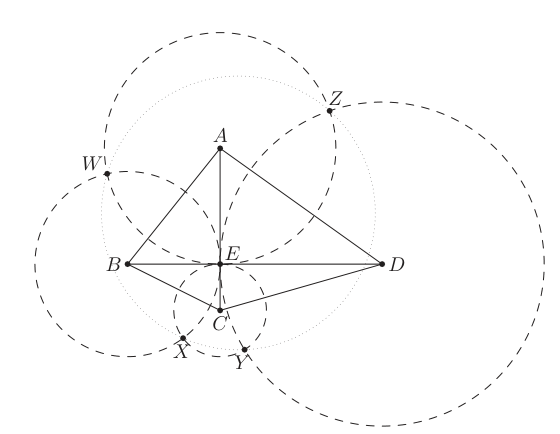
\includegraphics[width=0.6\linewidth]{USAMO1993Ori.png}
        \caption{../Gambar awal}
        \label{fig:USAMO1993Ori}
    \end{figure}

    Setelah dilakukan inversi terhadap titik $E$ (lebih lengkapnya, lingkaran yang berpusat di $E$ dan berjari-jari $1$), akan didapat konfigurasi yang ditunjukkan pada Figure \ref{fig:USAMO1993Inv}.
    \begin{figure}[h]
        \centering
        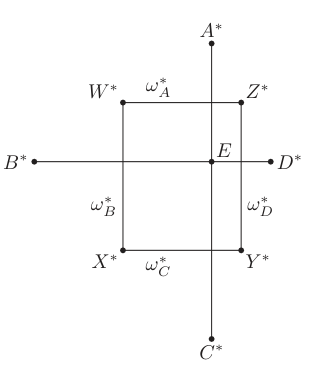
\includegraphics[width=0.3\linewidth]{USAMO1993Inv.png}
        \caption{../Gambar setelah diinversi}
        \label{fig:USAMO1993Inv}
    \end{figure}

    Dapat dicek bahwa keempat lingkaran yang berpusat di $A, B, C,$ dan $D$ akan dikirim menjadi garis yang secara berturut-turut tegak lurus dengan $EA, EB, EC,$ dan $ED$. Sehingga, $W^{*}X^{*}Y^{*}Z^*$ merupakan persegi panjang. Segiempat ini siklik sehingga sebelum diinversi sekalipun, $WXYZ$ haruslah merupakan segiempat siklik juga.
    
\end{proof}

\section{Pole-Polar}
Diberikan sebuah lingkaran $\omega$ yang berpusat di $O$ dan berjari-jari $R$. Misal $P^{*}$ adalah hasil inversi dari titik $P \neq O$ terhadap $\omega$. Garis $\ell$ yang melewati titik $P^{*}$ dan tegak lurus dengan $OP$ disebut sebagai \textbf{polar} dari $P$ dan sebaliknya, titik $P$ disebut sebagai \textit{pole} dari garis $\ell$.
\begin{figure}[h]
    \centering
    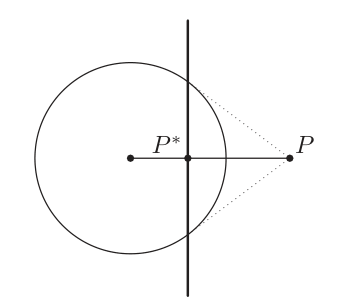
\includegraphics[width=0.5\linewidth]{PolePolar.png}
    \caption{Garis yang ada merupakan polar dari titik $P$}
    \label{fig:enter-label}
\end{figure}
Properti yang paling sering dipakai adalah sebagai berikut:
\begin{theorem}[Teorema La Hire]
    Diberikan lingkaran $\omega$. Titik $A$ dan $B$ secara berturut-turut adalah polar dari garis $a$ dan $b$. Maka, $A \in b$ jika dan hanya jika $B \in a$.
\end{theorem}
Terdapat kaitan antara pole-polar dan harmonic bundle:
\begin{lemma}
    \label{lemma:polar-harmonic}
    Diberikan lingkaran $\omega$ dengan tali busur $AB$. Titik $P$ dan $Q$ terletak di garis $AB$. Maka, $(A, B; P, Q) = -1$ jika dan hanya jika $P$ terletak di polar $Q$.
\end{lemma}
\begin{theorem}[Teorema Brocard]
    Diberikan segiempat siklik $ABCD$. Misal $P = AB \cap CD$, $Q = BC \cap DA$, dan $R = AC \cap BD$. Maka, $P, Q, R$ secara berturut-turut adalah pole dari $QR, RP, PQ$. Lebih lanjut, titik tinggi $PQR$ adalah titik pusat lingkaran luar $ABCD$.
\end{theorem}

Dua teorema lain yang tidak sebenarnya tidak terkait dengan pole-polar, inversi, atau harmonic bundle tetapi cukup berguna:
\begin{theorem}[Teorema Pascal]
    Diberikan segienam $ABCDEF$ siklik. Titik perpotongan $Ab \cap DE, BC \cap EF$, dan $CD \cap FA$ kolinear.
\end{theorem}

Ada banyak konfigurasi berbeda yang dapat dihasilkan Pascal seperti pada figure \ref{fig:pascal}. Bahkan beberapa titik dapat berhimpit menghasilkan segilima atau segiempat seperti pada figure \ref{fig:pascal-degen}.
\begin{figure}[h]
    \centering
    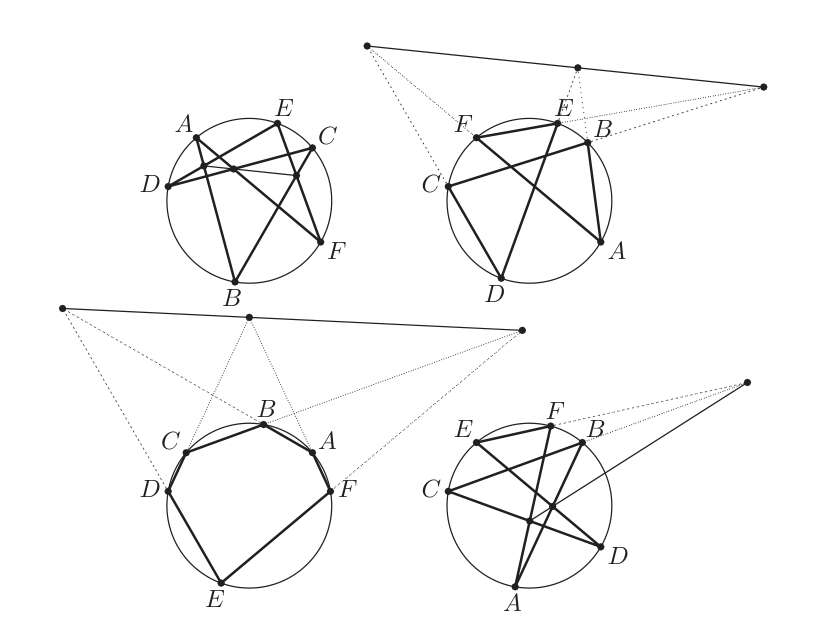
\includegraphics[width=0.7\linewidth]{Pascal.png}
    \caption{Berbagai konfigurasi Teorema Pascal}
    \label{fig:pascal}
\end{figure}

\begin{figure}[h]
    \centering
    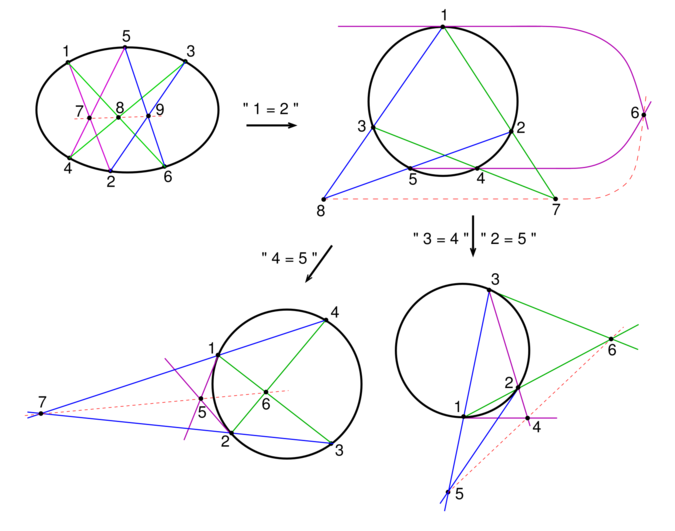
\includegraphics[width=0.7\linewidth]{PascalDegenerate.png}
    \caption{Pascal degenerate cases}
    \label{fig:pascal-degen}
\end{figure}

\begin{theorem}
    (Teorema Brianchon) Diberikan sebuah segienam $ABCDEF$ dengan lingkaran dalam. Maka, $AD, BE,$ dan $CF$ konkuren.
\end{theorem}
Sama seperti sebelumnya, urutan titik-titik ini dapat diubah-ubah dan juga dapat dibuat versi degeneratenya.
\section{Contoh Soal}
\begin{example}
    Diberikan sebuah segitiga $ABC$. Jika $D, E, F$ secara berturut-turut merupakan titik singgung lingkaran dalam $ABC$ ($\omega$) terhadap sisi $BC, CA, AB$. Titik $I$ adalah titik pusat lingkaran dalam $ABC$. Garis $EF$ dan $BC$ berpotongan di titik $K$. Buktikan bahwa $IK \perp AD$.
\end{example}

\begin{proof}[Solusi:]
    Misal $X = EF \cap \omega$. Tinjau inversi terhadap $\omega$. Karena $AF$ dan $AE$ keduanya merupakan garis singgung terhadap $\omega$, didapat $FE$ merupakan polar dari $A$. Teorema La Hire menyatakan bahwa $K \in FE$ yang merupakan polar $A$ mengakibatkan $A$ ada di polar $K$. Polar dari $K$ adalah garis $DX'$ dengan $X$ adalah titik di $\omega$ selain $D$ sehingga $KX$ menyinggung $\omega$. Namun, karena $A, D, X$ segaris dan $A, D, X'$ juga segaris serta $X'$ harus ada di keliling $\omega$, maka $X = X'$. Sehingga, $KX$ adalah garis singgung $\omega$ dan $IK$ tegak lurus $XD$.
\end{proof}

\section{Soal}
\begin{problem}
    (IMO SL 1989) Sebuah segiempat $ABCD$ siklik dengan lingkaran luarnya berpusat di $O$. Selain itu, segiempat $ABCD$ memiliki lingkaran dalam yang menyinggung keempat sisinya dan berpusat di titik $I$. Jika $E = AC \cap BD$, buktikan bahwa $E, I, O$ segaris. \textbf{Hint: Romania}
\end{problem}

\begin{problem}
    Diberikan lingkaran $\omega_1, \omega_2,$ dan $\omega_3$ yang berpotongan di satu titik $O$. Diketahui bahwa $\omega_1 \cap \omega_2 = \{O, C\}$, $\omega_2 \cap \omega_3 = \{O, A\}$, dan $\omega_3 \cap \omega_1 = \{O, B\}$. Lebih lanjut, $AO \cap \omega_1 = \{O, D\}$, $BO \cap \omega_2 = \{O, E\}$, dan $CO \cap \omega_3 = \{O, F\}$. Jika diketahui bahwa $OE$ dan $OF$ secara berturut-turut adalah diameter $\omega_2$ dan $\omega_3$, buktikan bahwa $OD$ adalah diameter $\omega_1$. \textbf{Hint: Republik Afrika Tengah} 
\end{problem}

\begin{problem}
    Lingkaran $\omega_1$ dan $\omega_2$ bersinggungan secara eksternal di titik $A$. Sebuah garis singgung persekutuan menyinggung $\omega_1$ di $P$ dan $\omega_2$ di $Q$. Garis singgung persekutuan lain menyinggung $\omega_1$ di $R$ dan $\omega_2$ di $S$. Buktikan bahwa lingkaran luar segitiga $APQ$ dan lingkaran luas segitiga $RAS$ bersinggungan secara eksternal. \textbf{Hint: Peru}
\end{problem}

\begin{problem}
    Lingkaran $\omega_1$, $\omega_2$, $\omega_3$, dan $\omega_4$ adalah empat lingkaran yang bersinggungan secara eksternal di titik $A$, $B$, $C$, $D$ seperti yang ditunjukkan pada figure \ref{fig:evan-chen-8.24}. Buktikan bahwa $ABCD$ adalah segiempat siklik. \textbf{Hint: Peru, Georgia}
    \begin{figure}[h]
        \centering
        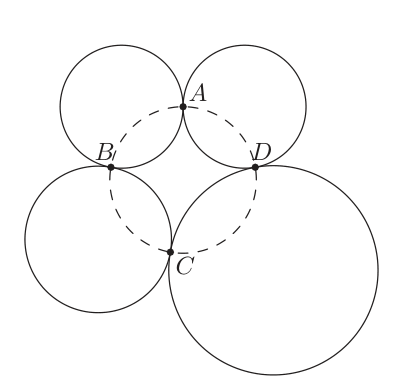
\includegraphics[width=0.5\linewidth]{EvanChen8.24.png}
        \caption{$ABCD$ siklik}
        \label{fig:evan-chen-8.24}
    \end{figure}
\end{problem}

\begin{problem}
    (Tugas Pembinaan Jarak Jauh IMO 2018) Pada sebuah segiempat konveks $ABCD$ kedua diagonal $AC$ dan $BD$ berpotongan di $O$. Titik $A_1,B_1,C_1,D_1$ berturut-turut terletak pada segmen $AO,BO,CO,$ dan $DO$ sedemikian sehingga $AA_1=CC_1$ dan $BB_1=DD_1$. Misalkan $M\neq O$ merupakan titik perpotogan dari lingkaran luar  $\triangle AOB$ dan  $\triangle COD$. Misalkan $N\neq O$ merupakan titik potong  lingkaran luar $\triangle AOD$ dan $\triangle BOC$; $P\neq O$ titik  perpotongan lingkaran luar $\triangle A_1OB_1$ dan $\triangle C_1OD_1$, dan $Q\neq O$ titik potong lingkaran luar $\triangle A_1OD_1$ dan $\triangle B_1OC_1$. Buktikan bahwa $MNPQ$ merupakan sebuah segiempat talibusur. \textbf{Hint: Republik Afrika Tengah, Palau}
\end{problem}

\newpage
\section{Hint}
\begin{enumerate}
    \item (Bangui) Inversi terhadap $O$
    \item (Bucharest) Brianchon dan Brocard
    \item (Lima) Inversi terhadap $A$
    \item (Ngerulmud) Buktikan bahwa $MNOP$ siklik
    \item (Tbilisi) Buktikan bahwa $B^*, C^*, D^*$ segaris
\end{enumerate}
\end{document}